\subsection{Добавляем нейтральные города}
Добавим в шаблон нейтральные города. В качестве примера будем создавать разное количество городов в зависимости от размера сценария: один город для размера 48 и два города для 72. Сценарий размера 48 будет содержать город Т2, а сценарий 72 города Т3 и Т5.

Поскольку правило одинаково для двух зон опишем логику городов также отдельной функцией с названием \texttt{getTowns}. Согласно описанию зоны, поле \texttt{towns} представляет собой \textbf{список} описаний городов. В нашем случае список будет содержать одно описание для сценария размером 48 и два описания для 72:

\begin{figure}[H]
\lstinputlisting[firstnumber=1, firstline=1, lastline=12]{docExamples/templateExample4.lua}
\end{figure}

Авторы шаблонов в праве выносить логику в функции и называть их по своему усмотрению.

Не забываем вызывать нашу новую функци в описаниях стартовых зон, передавая размер сценария выбранный пользователем:

\begin{figure}[H]
\lstinputlisting[firstnumber=54, firstline=54, lastline=54]{docExamples/templateExample4.lua}
\lstinputlisting[firstnumber=63, firstline=63, lastline=63]{docExamples/templateExample4.lua}
\end{figure}

Поскольку в описаниях городов отсутствуют гарнизоны, посещающие отряды или лут, мы получаем пустые города как и ожидалось:

\begin{figure}[H]
\center
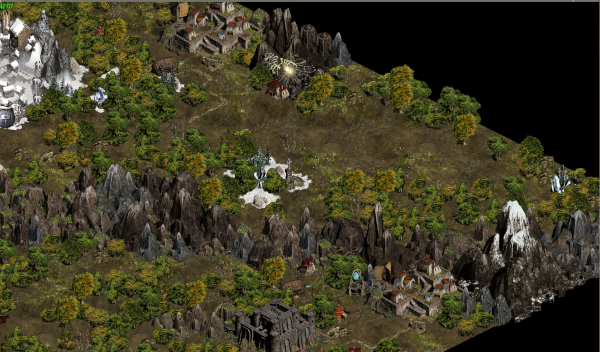
\includegraphics[width=1.0\linewidth]{docImages/scenario48Towns.png}
\caption{Города в сценарии размером 48}
\end{figure}

\begin{figure}[H]
\center
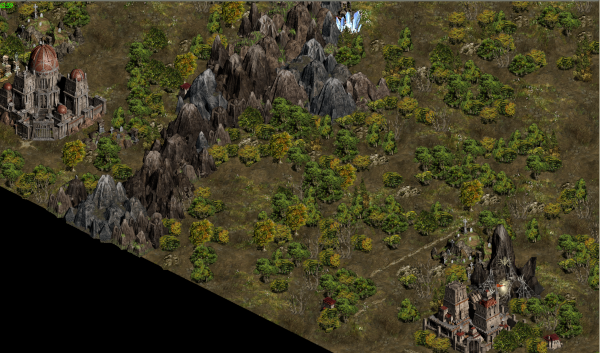
\includegraphics[width=1.0\linewidth]{docImages/scenario72Towns.png}
\caption{Города в сценарии размером 72}
\end{figure}

Теперь когда мы убедились в правильности нашей логики для двух размеров сценариев, можно добавить в города охрану и награды. В гарнизоне Т2 города может быть максимум 2 юнита, посадим туда волков и зеленокожих общей ценностью 200 опыта:

\begin{figure}[H]
\lstinputlisting[firstnumber=4, firstline=4, lastline=11]{docExamples/templateExample5.lua}
\end{figure}

В город Т3 добавим посещающий отряд из варваров и нейтральных людей на 500 опыта, а гарнизон оставим пустым. В качестве награды за захват города положим в инвентарь гарнизона 3 - 4 эликсира восстановления (лечение на 100 хп):

\begin{figure}[H]
\lstinputlisting[firstnumber=13, firstline=13, lastline=26]{docExamples/templateExample5.lua}
\end{figure}

Как упоминалось в самом начале, порядок задания полей в таблицах не играет роли.

В город Т5 добавим отряд из нейтральных людей и эльфов на 500 опыта, а защитников в гарнизоне выберем из жителей болот и нейтралов. Тоже на 500 опыта. В качестве награды посещающий отряд будет владеть одним эликсиром всевышнего (+10\% хп перманентно). В инвентарь гарнизона положим драгоценностей общей суммой 2000 и диапазоном ценности каждой вещи от 250 до 750 золотых. На моде Мотлина версии 1.5.3 такой диапазон ценности должен наполнить инвентарь гарнизона бронзовыми и серебряными кольцами, а также изумрудами. Других типов драгоценностей в награде быть не должно:

\begin{figure}[H]
\lstinputlisting[firstnumber=28, firstline=28, lastline=48]{docExamples/templateExample5.lua}
\end{figure}

Проверим результаты создав сценарий размером 72.\\
Города Т3:

\begin{figure}[H]
\begin{center}
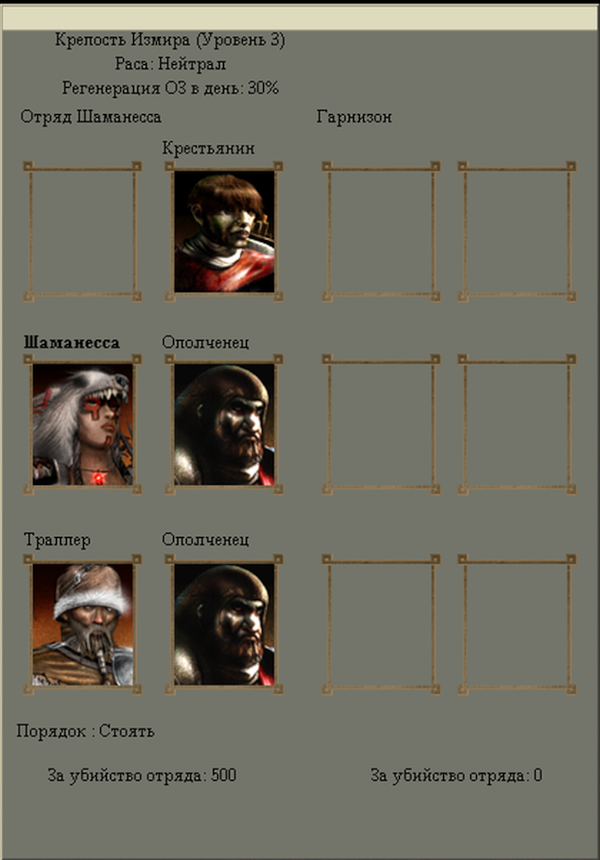
\includegraphics[width=.45\linewidth]{docImages/townT3Preview.png}
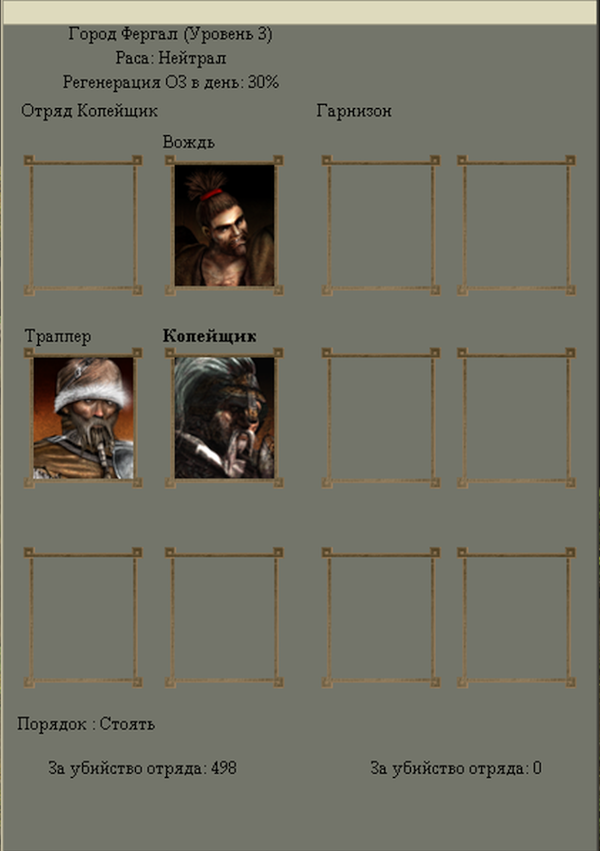
\includegraphics[width=.45\linewidth]{docImages/townT3Preview2.png}
\caption{Просмотр Т3 городов}
\end{center}
\end{figure}

Информация об опыте за убийство отрядов говорит нам о том, что посещающие отряды сгенерировались корректно: близко к 500 опыта в сумме и с учетом заданных субрас.

Проверим инвентари городов:

\begin{figure}[H]
\center
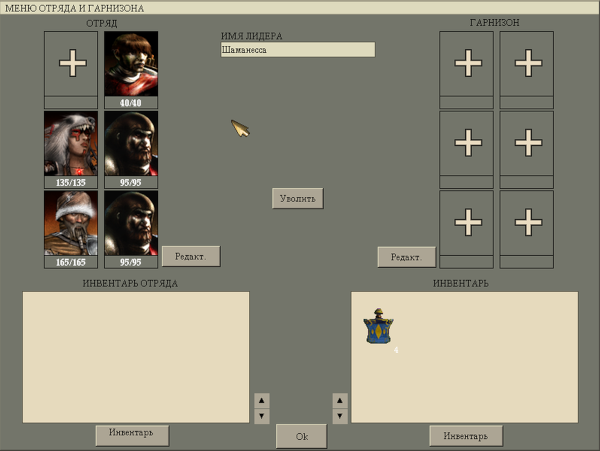
\includegraphics[width=1.0\linewidth]{docImages/townT3Loot.png}
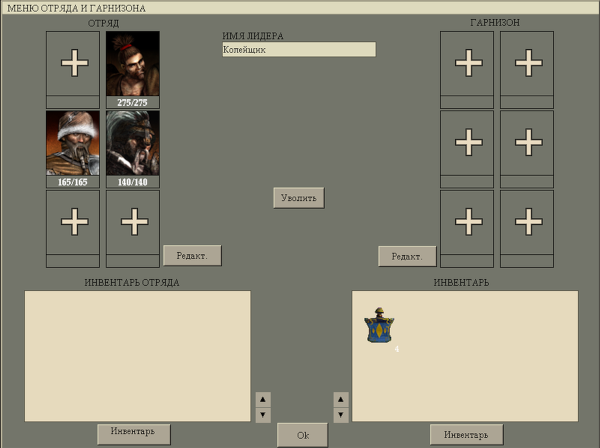
\includegraphics[width=1.0\linewidth]{docImages/townT3Loot2.png}
\caption{Награды Т3 городов}
\end{figure}

Эликсиры восстановления лежат в инвентарях гарнизонов, как и было задумано в шаблоне.

Проверим результаты генерации Т5 городов:

\begin{figure}[H]
\begin{center}
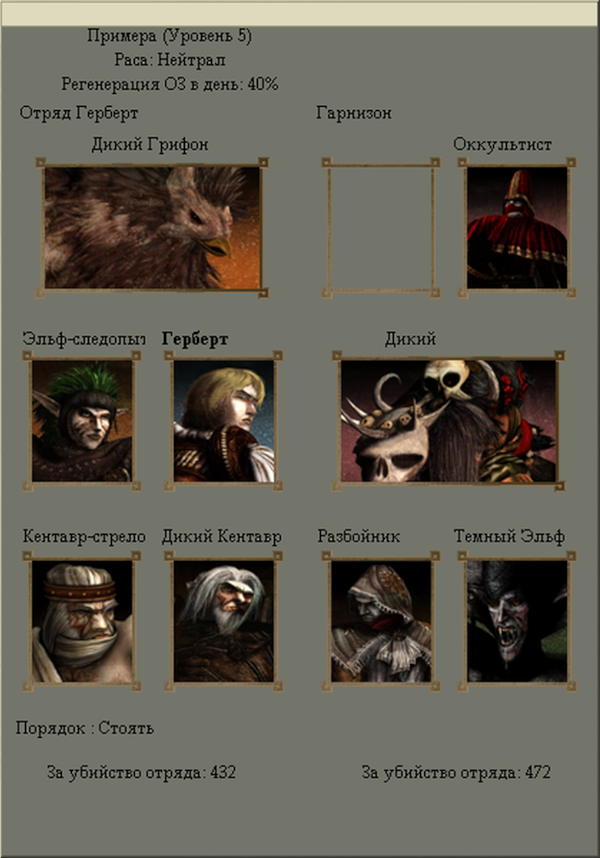
\includegraphics[width=.45\linewidth]{docImages/townT5Preview.png}
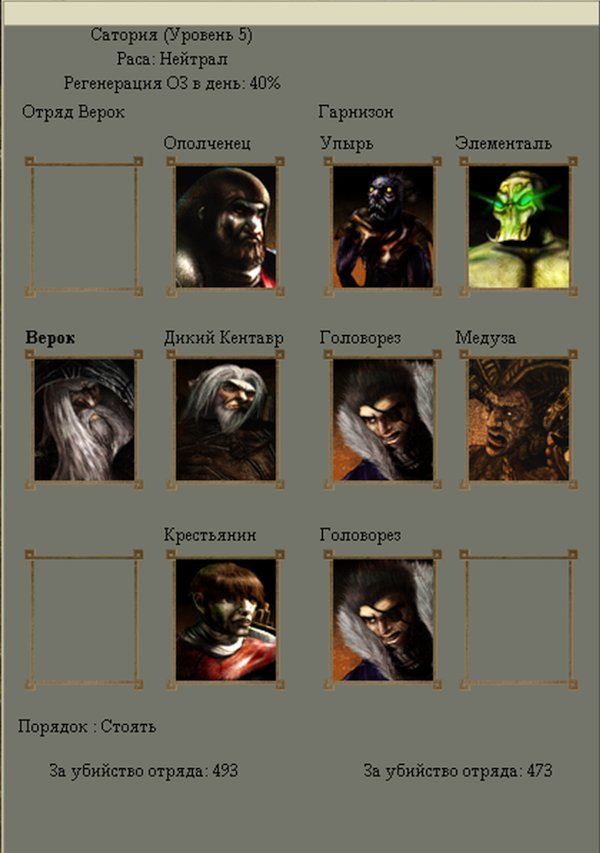
\includegraphics[width=.45\linewidth]{docImages/townT5Preview2.png}
\caption{Просмотр Т5 городов}
\end{center}
\end{figure}

Есть небольшой разброс ценности, но отряды и их субрасы созданы согласно описанию шаблона.

Смотрим инвентари Т5 городов:

\begin{figure}[H]
\center
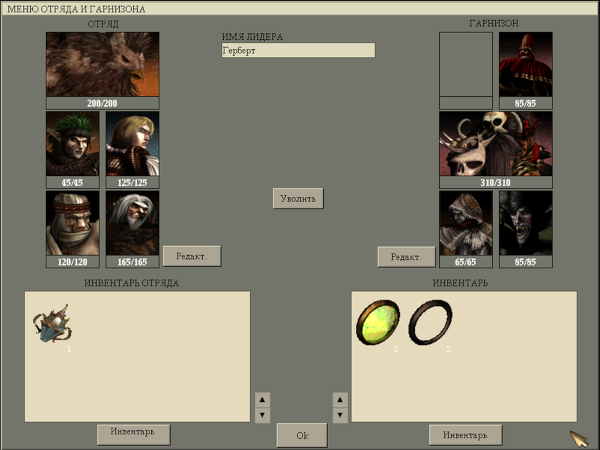
\includegraphics[width=1.0\linewidth]{docImages/townT5Loot.png}
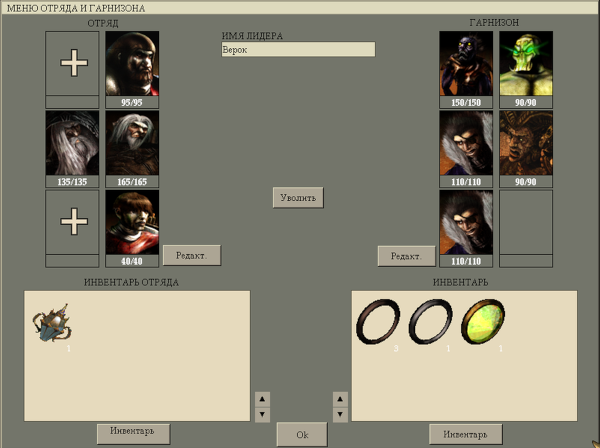
\includegraphics[width=1.0\linewidth]{docImages/townT5Loot2.png}
\caption{Награды Т5 городов}
\end{figure}

Как видим перманентные зелья на месте, а драгоценности в гарнизонах собраны лишь из двух видов колец и изумрудов в случайных пропорциях, но согласно общей сумме. Все согласно описанию шаблона.

Полный текст функции \texttt{getTowns}:

\begin{figure}[H]
\lstinputlisting[firstnumber=1, firstline=1, lastline=52]{docExamples/templateExample5.lua}
\end{figure}

Полный текст шаблона, а также другие примеры шаблонов идут вместе с программой генератора и этой документацией.